\section{Event selection and background estimation}
\label{s:selection}

Only events collected using single-electron or single-muon triggers are
accepted. The trigger thresholds,  $\pT > 24\,\GeV$ for electrons and
 $\pT > 20\,\GeV$ for muons, are set to be almost fully efficient for
reconstructed leptons with $\pT > 25\,\GeV$.  Events are required
to have at least one reconstructed primary vertex.  In all selections
considered, at least one reconstructed lepton with $\pT > 25\,\GeV$ is required
to match ($\Delta R_{\eta} < 0.15$) a lepton with the same flavour
reconstructed by the trigger algorithm.  Three channels are defined based on
the number of reconstructed leptons, which are sorted according to their
transverse momentum in decreasing order. 
%A subset of the sensitive signal regions in the Run-1 analysis~\cite{TOPQ-2013-05} is used, with very similar definitions.

Background events containing well-identified prompt leptons are modelled by simulation. The
normalisations for the $WZ$ and $ZZ$ processes are taken from data control regions and 
included in the fit.
The yields in these data control regions are 
extrapolated to the signal regions using simulation.
Systematic uncertainties in the extrapolation are taken into account in the
overall uncertainty in the background estimate.

Background sources involving one or more fake leptons are modelled 
using data events from control regions.  For the same-sign dimuon (\SSLSR) analysis and the
trilepton analysis the fake-lepton background is estimated using the matrix
method~\cite{TOPQ-2010-01}, where any combination of fake leptons among the
selected leptons is considered.  However, compared to Ref.~\cite{TOPQ-2010-01}, the 
real- and fake-lepton efficiencies used by the matrix method are estimated
in a different way in this measurement. The lepton efficiencies are measured by
applying the matrix method in control regions, where the lepton efficiencies
are extracted in a likelihood fit as free parameters using the matrix method
as model, assuming Poisson statistics, and assuming that events with two fake
leptons are negligible. In this way the parameters are by construction the
actual parameters of the matrix model itself, instead of relying on external
lepton efficiency measurements which are not guaranteed to be fully consistent
with the matrix model.
The
control regions are defined in dilepton events, separately for $b$-tagged and
$b$-vetoed events to take into account the different fake-lepton efficiencies
depending on whether the source is a light-flavour jet or a heavy-flavour jet.
The real-lepton efficiencies are measured in inclusive opposite-sign events,
and fake-lepton efficiencies in events with same-sign leptons and $\met>40\,\GeV$
(for $b$-tagged events $\met>20\,\GeV$), after subtracting the estimated
contribution from events with misidentification of the charge of a lepton
(referred to as ``charge-flip'' in the following), and excluding the same-sign dimuon signal region. The charge-flip events are subtracted using simulation. The
extracted fake-lepton efficiencies are found to be compatible with fake-lepton
efficiencies from a fully data-driven procedure where the charge-flip events
are estimated from data.  For the \FLC, the contribution from backgrounds
containing fake leptons is estimated from simulation and corrected with scale
factors determined in control regions.

The full selection requirements and the background evaluation strategies in the
different channels are described below.

\subsection{Same-sign dimuon analysis}

The same-sign dimuon signal region targets the \ttW process and has
the highest sensitivity among all same-sign dilepton
regions~\cite{TOPQ-2013-05}.  The main reason for this is that electrons have a
much larger charge misidentification probability, inducing a significant
background from top-quark pairs.  Events are required to have two muon
candidates with the same charge and $\pt>25\,\GeV$, $\met > 40\,\GeV$, the scalar
sum of the \pT of selected leptons and jets, \HT, above $240\,\GeV$, and at least
two $b$-tagged jets. Events containing additional leptons (with $\pT>7\,\GeV$)
are vetoed.

The dominant background in the \SSLSR\ region arises from events containing
fake leptons, where the main source is \ttbar events. Backgrounds from the
production of prompt leptons with correctly
identified charge come primarily from $WZ$ production, but the relative
contribution of this background is small compared to the fake-lepton
background. The charge-flip background is negligible in this signal region, as
the probability of misidentifying the charge of a muon in the relevant \pT
range is negligible.  
For the validation of the fake-lepton background estimate a region is defined
based on the signal region selection but omitting the \met requirement,
reducing the \pT threshold of the subleading lepton to $20\,\GeV$ and requiring 
at least one $b$-tagged jet.
The distributions of \met and subleading lepton \pT in this validation region ($2\mu$-SS-VR) are shown in
Figure \ref{fig:ssmm_val}.  The expected numbers of events in the \SSLSR\
signal region are shown in Table~\ref{tab:yields}. Nine events are
observed in data for this signal region.
 

\begin{figure}[htbp]
\centering
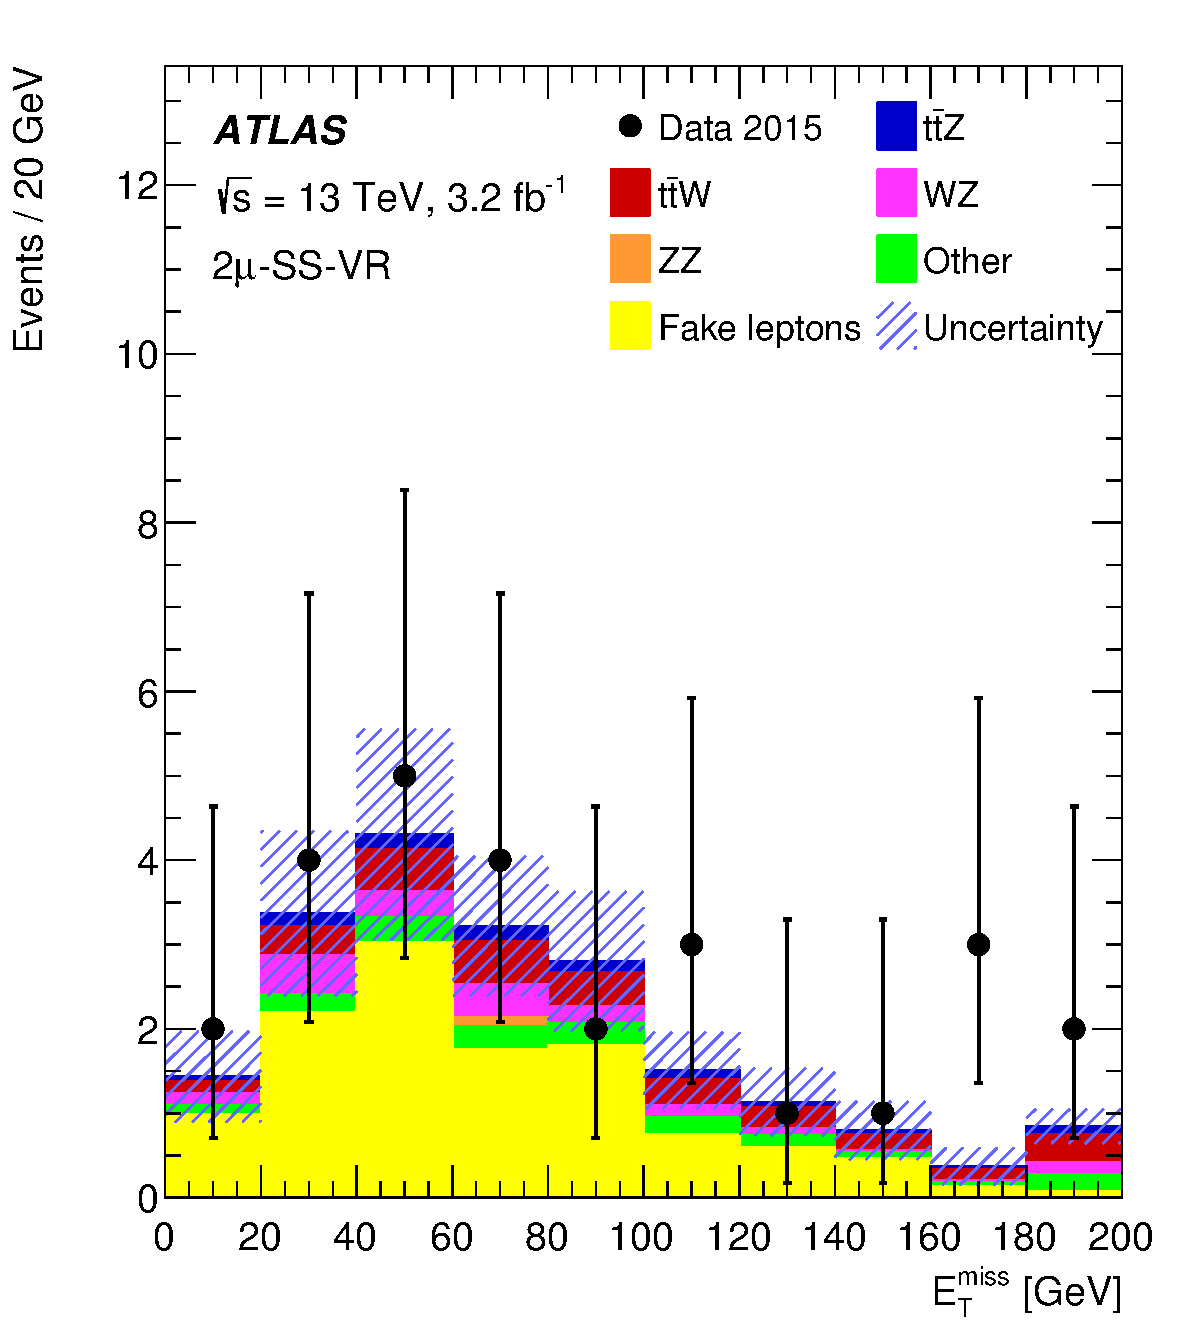
\includegraphics[width=\twofigwidth]{SS2mu1b_MET}
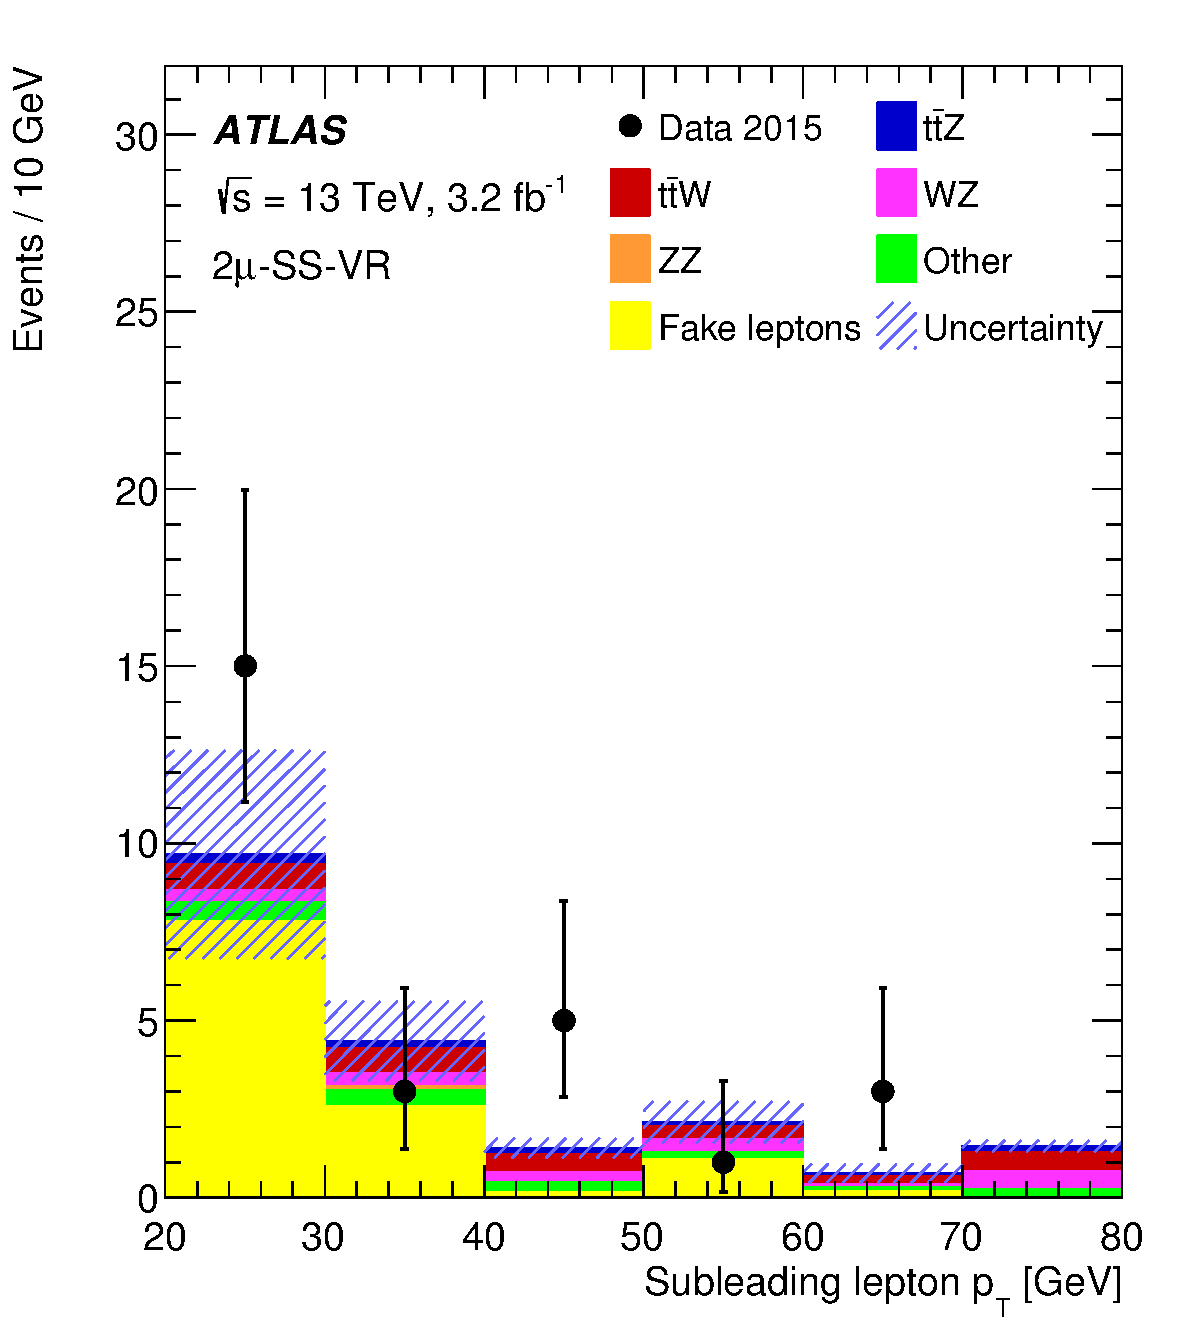
\includegraphics[width=\twofigwidth]{SS2mu1b_pT_2lep}
\caption{\label{fig:ssmm_val} (Left) The \met and (right) subleading lepton \pT 
distributions shown for the $b$-tagged \SSLSR\ channel where the signal region
requirements on subleading lepton \pT, number of $b$-tags, and \met are
relaxed. \hatch.  The background denoted `Other' contains other SM processes
producing two same-sign prompt leptons.  \oflo.} 
\end{figure}

\subsection{Trilepton analysis}

Four signal regions with exactly three leptons are considered.  The first three
are sensitive to \ttZ; each of these requires an opposite-sign same-flavour
(OSSF) pair of leptons whose invariant mass is within $10\,\GeV$ of the $Z$ boson mass.
The signal regions are categorised by their jet and $b$-jet multiplicities and
have different signal-to-background ratios.  In the \TLSRA\ region, at least
four jets are required, exactly one of which is $b$-tagged. In the \TLSRB\
region, exactly three jets with at least two $b$-tagged jets are required.  In
the \TLSRC\ region, at least four jets are required, of which at least two are
$b$-tagged. 

In the \TLSRD\ region at least two and at most four jets are required, of which
at least two are $b$-tagged, no OSSF lepton pair is allowed in the $Z$
boson mass window, and the sum of the lepton charges must be $\pm$1.  This region
primarily targets the \ttW process but also has a sizeable \ttZ contribution.

The signal region definitions for the \TLC\ are summarised
in Table~\ref{tab:SRs3l}, while the expected numbers of events in the signal
regions are shown in Table~\ref{tab:yields}.  The dominant backgrounds in the
\TLSRA, \TLSRB\ and \TLSRC\ signal regions arise from $Z$+jets production with
a fake lepton, diboson production and the production of a single top quark in
association with a $Z$ boson.

\begin{table}[htbp]
\centering
\caption{Summary of event selections in the trilepton signal regions.\vspace{1ex}} 
\label{tab:SRs3l}
\begin{tabular}{l|c|c|c|c}
\toprule
Variable  & \TLSRA & \TLSRB & \TLSRC & \TLSRD\\
\midrule
Leading lepton & \multicolumn{4}{c}{$\pT>25\,\GeV$} \\
Other leptons & \multicolumn{4}{c}{$\pT>20\,\GeV$} \\
Sum of lepton charges &  \multicolumn{4}{c}{$\pm1$} \\
$Z$-like OSSF pair & \multicolumn{3}{c|}{$|m_{\ell\ell} - m_Z| < 10\,\GeV$} & $|m_{\ell\ell} - m_Z| > 10\,\GeV$\\ 
$n_{\text{jets}}$ & $\ge 4$ & $3$ &  $\ge 4$ & $\ge2$ and $\le4$\\
$n_{b{\text{-jets}}}$ & $1$ & $\ge2$ & $\ge2$ & $\ge2$\\
\bottomrule
\end{tabular}
\end{table}

A control region is used to constrain the normalisation of the $WZ$ background
in data. Exactly three leptons are required, at least one pair of which must 
be an OSSF pair with an invariant mass within $10\,\GeV$ of the $Z$ boson mass. 
There must be exactly three jets,
none of which pass the $b$-tagging requirement.  With these requirements, the
expected \ttZ signal contribution is roughly 1\% of the total number of events.
This region is referred to as \TLCR\ and it is included in the fit. Distributions
comparing data and SM prediction are shown in Figure~\ref{fig:3l_wzcr}.

\begin{figure}[htbp]
\centering
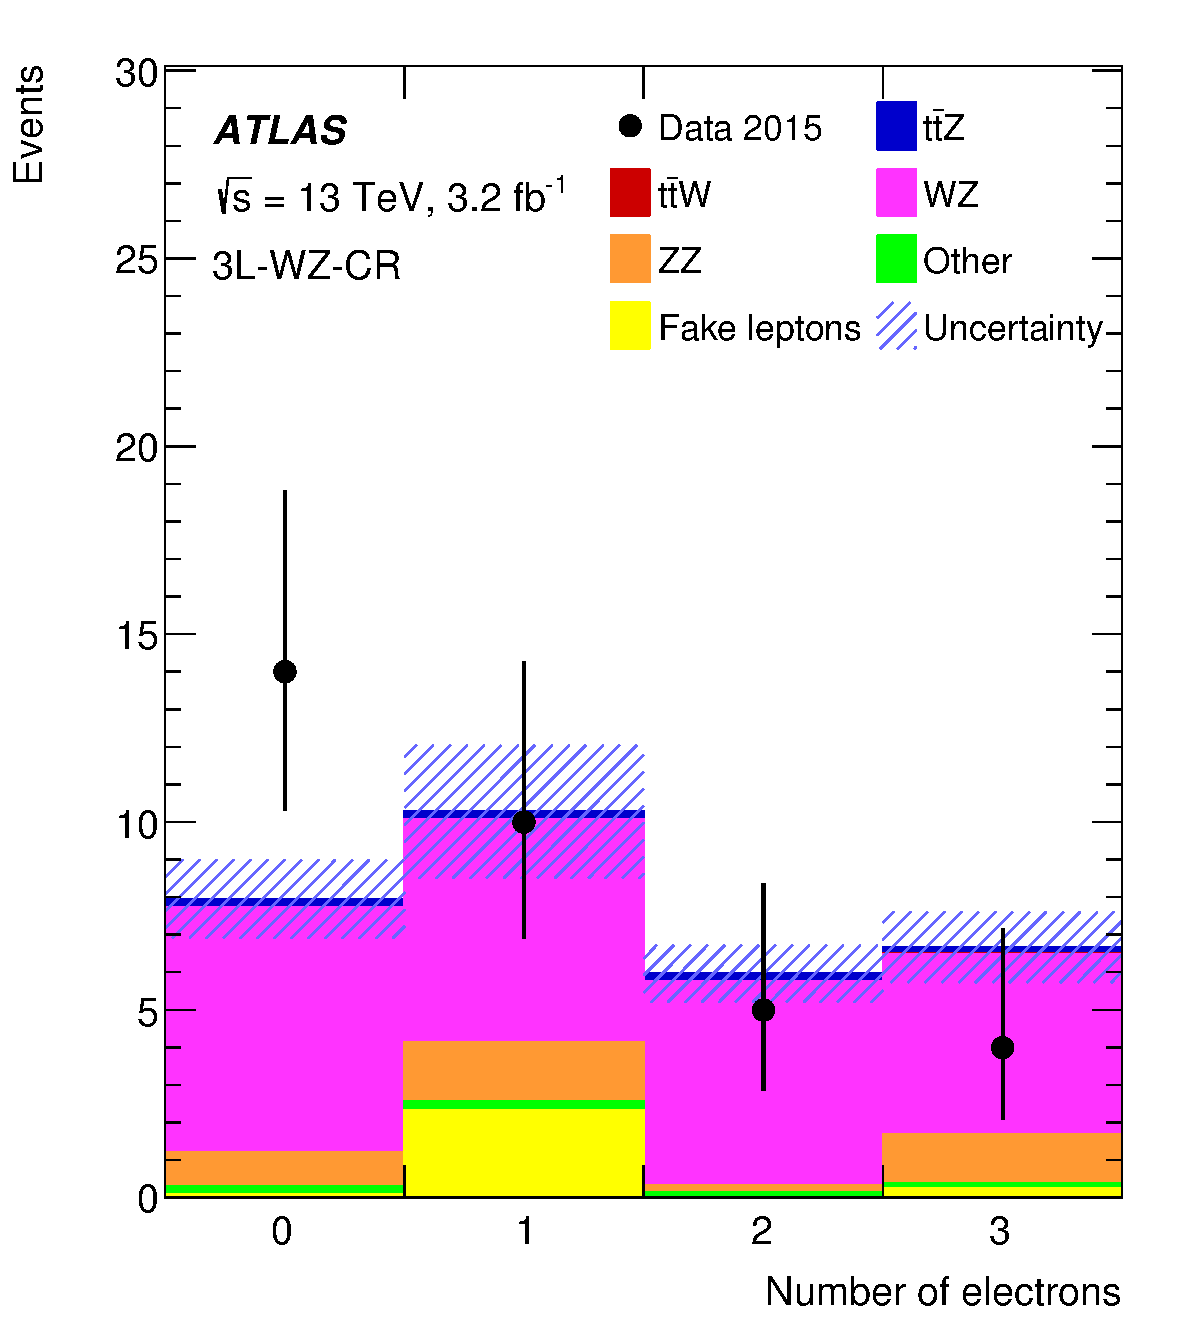
\includegraphics[width=\twofigwidth]{CRWZnEl}
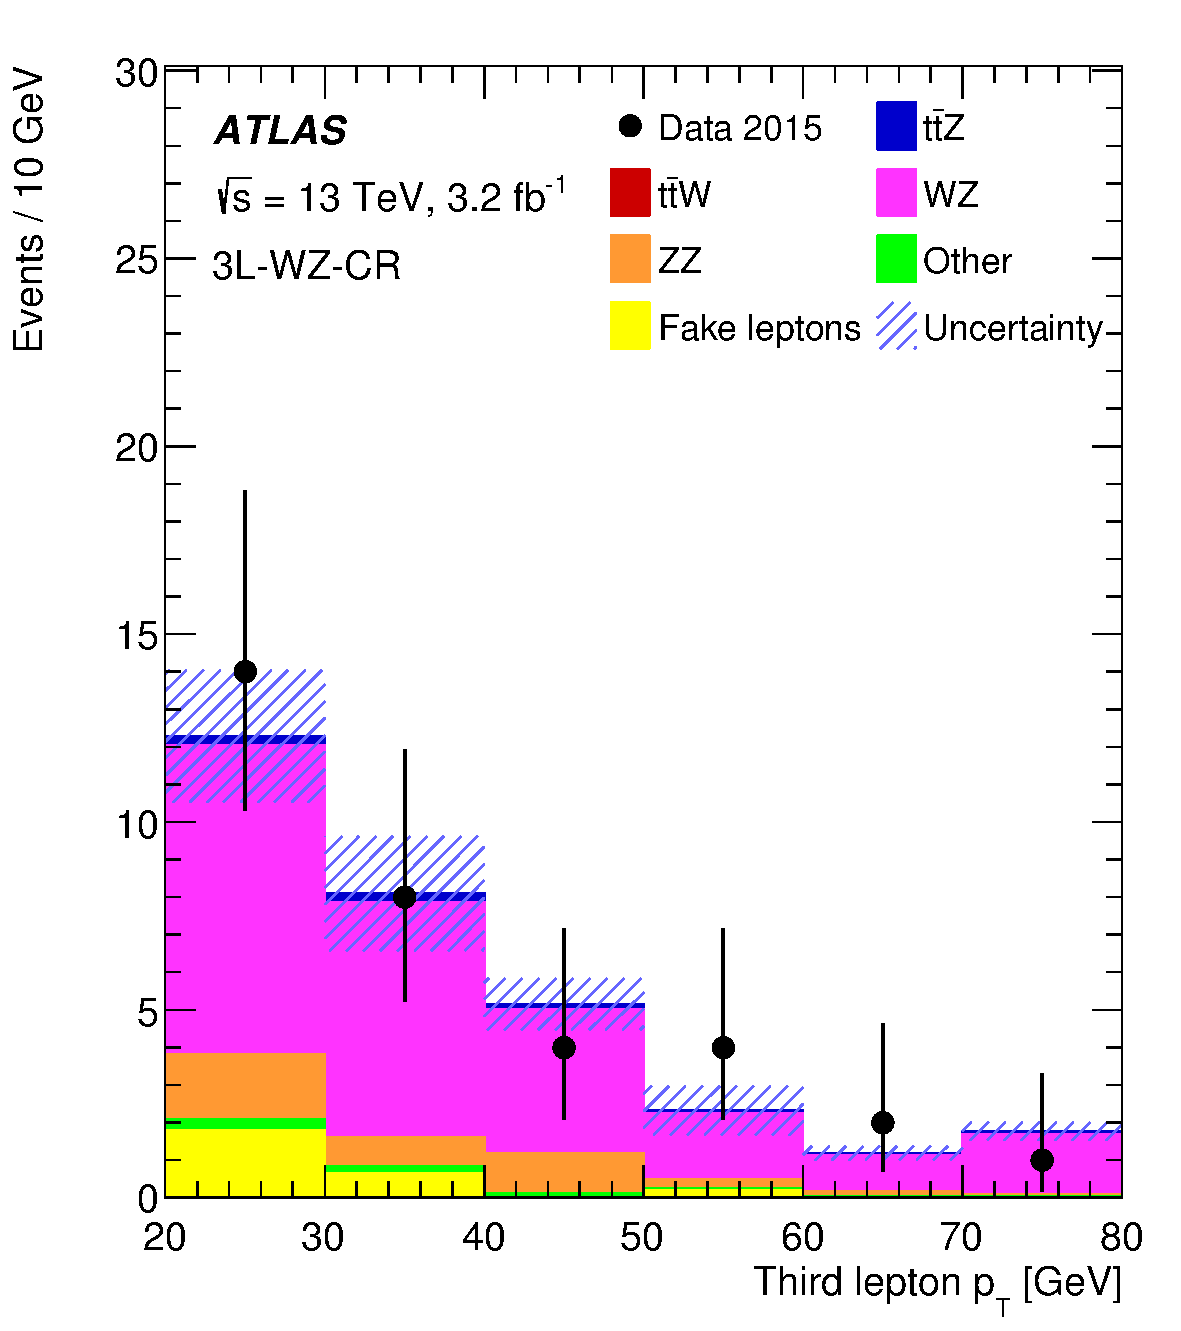
\includegraphics[width=\twofigwidth]{CRWZpT3lep}
\caption{\label{fig:3l_wzcr} Distributions of (left) the number of electrons
and (right) the third-lepton \pt in the \TLCR\ control region before the fit.  
The background
denoted `Other' contains other SM processes producing three prompt leptons.
\hatch. \oflor.}
\end{figure}

Two background validation regions are defined for the \TLC.  In the first
region, $3\ell$-Z-VR, the presence of two OSSF leptons with an invariant mass
within $10\,\GeV$ of the mass of the $Z$ boson is required.  The region requires
the events to have at most three jets where exactly one is $b$-tagged, or
exactly two jets where both jets are $b$-tagged.  The main backgrounds are $WZ$
production and $Z$+jets events with fake leptons.  In the second region,
$3\ell$-noZ-VR, events with such a pair of leptons are vetoed.  This region
requires the events to have at most three jets where exactly one is $b$-tagged,
and it is dominated by the fake-lepton background from top-quark pair production.
Neither validation region is used in the fit.  The distributions of the number
of electrons in each of the two validation regions are shown in
Figure~\ref{fig:3l_val}, demonstrating that data and background modelling are 
in good agreement within statistical uncertainties.

\begin{figure}[htbp]
\centering
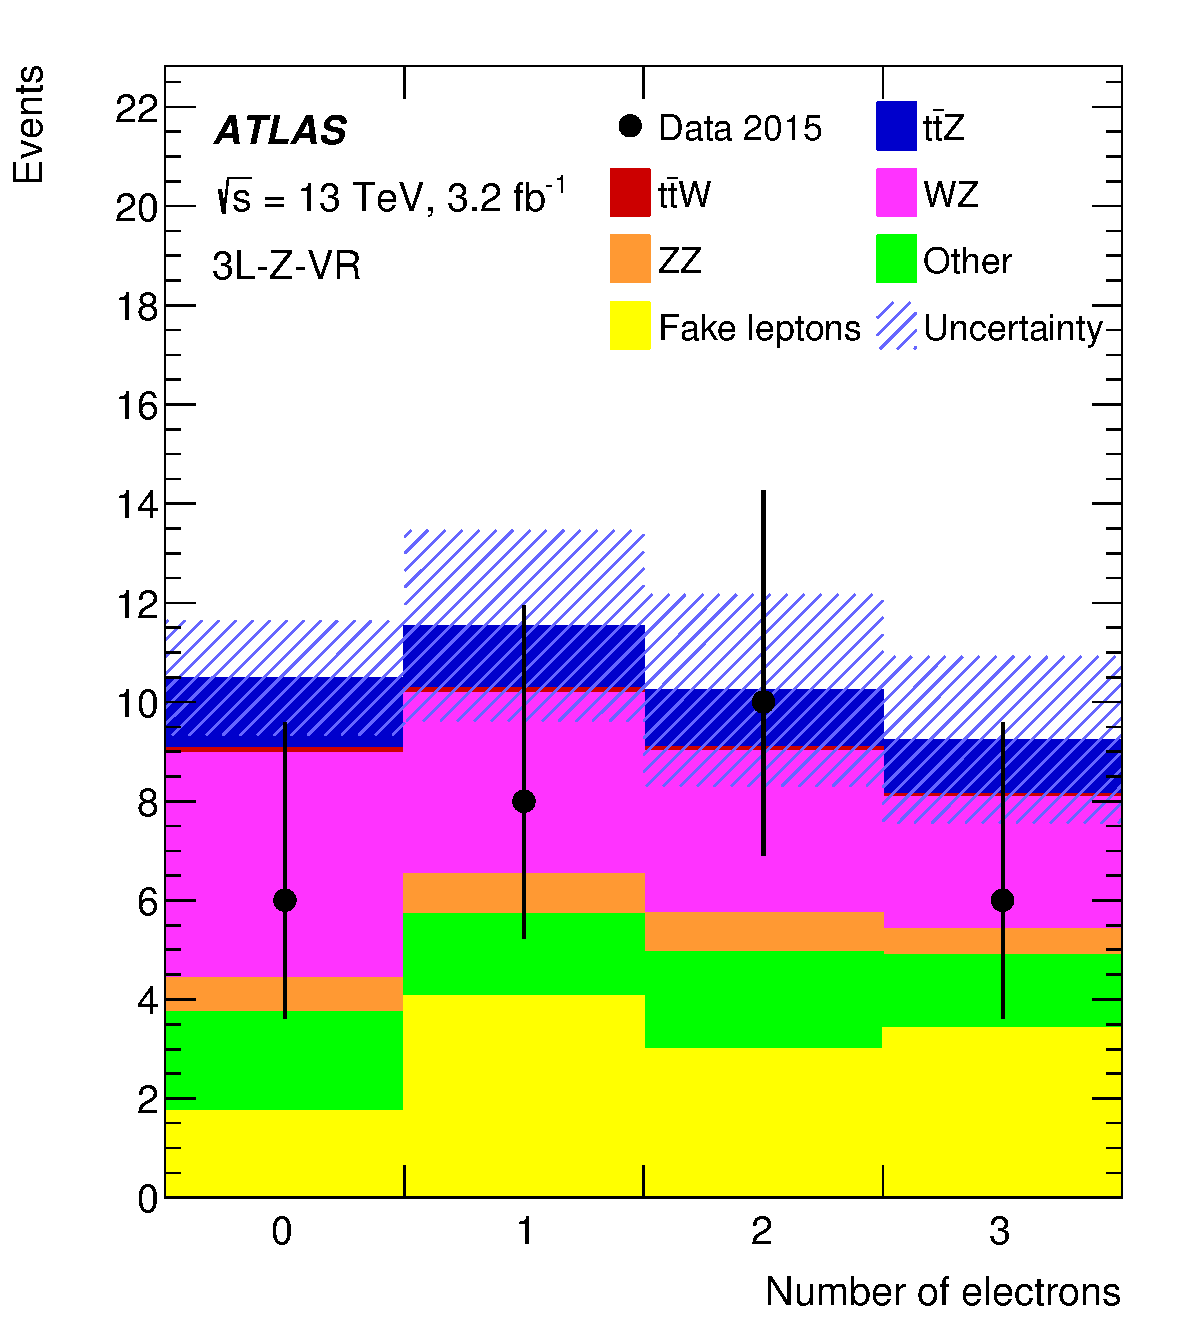
\includegraphics[width=\twofigwidth]{VR3lZ_nEl}
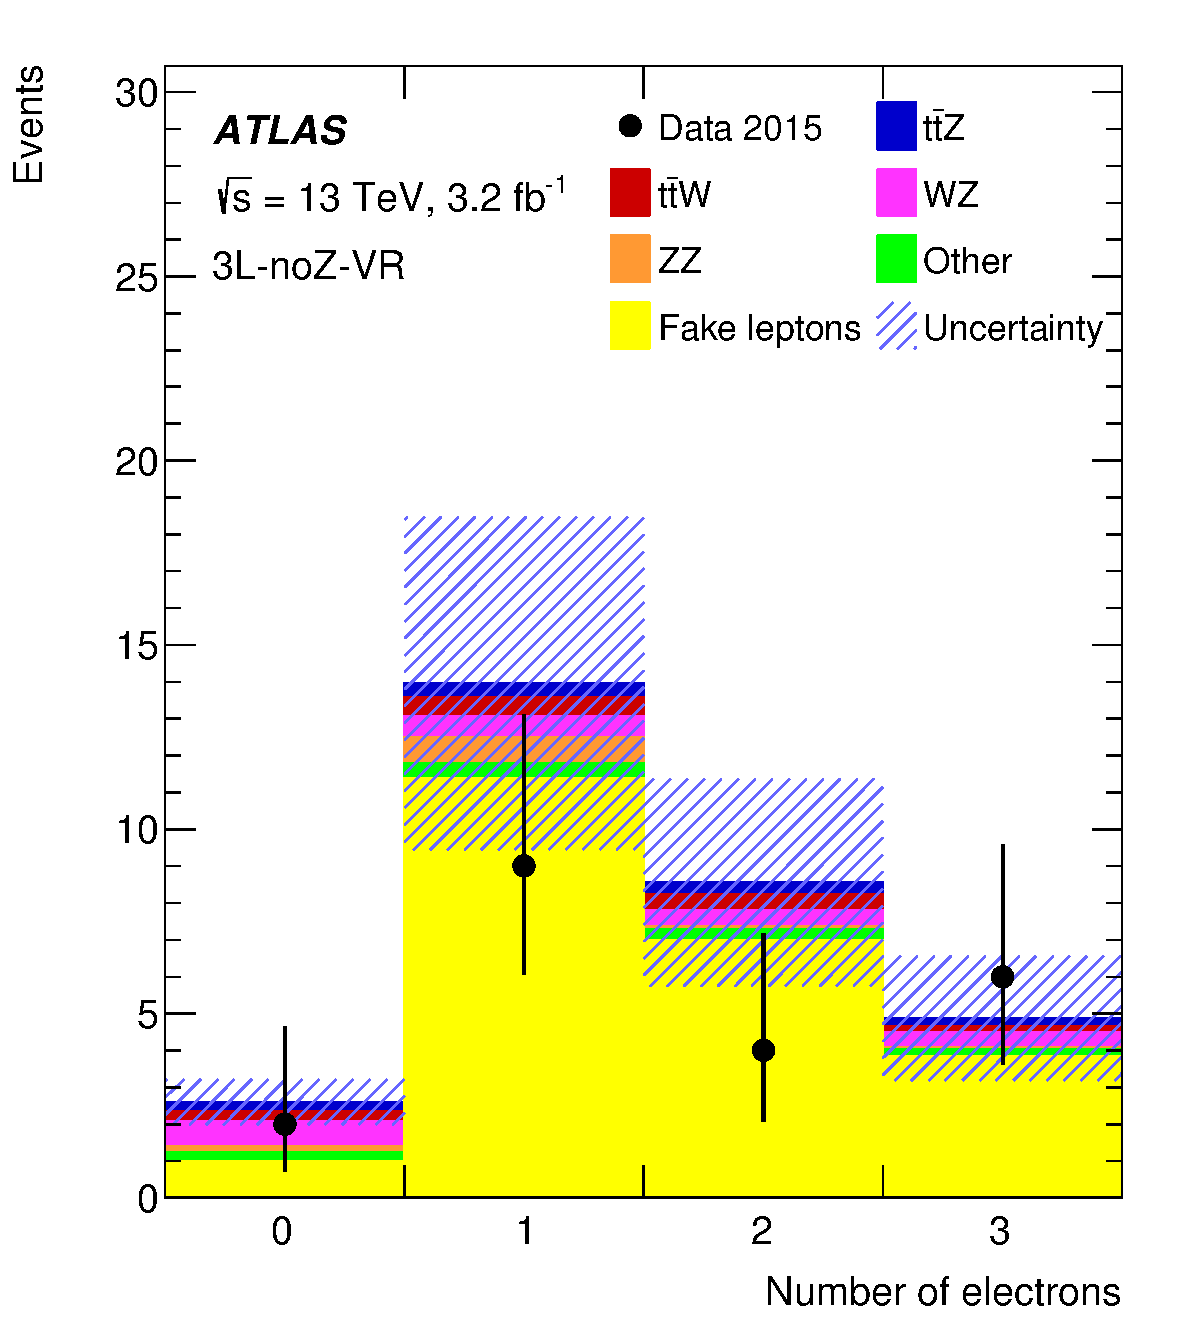
\includegraphics[width=\twofigwidth]{VR3lnoZ_nEl}
\caption{\label{fig:3l_val} Distributions of the number of electrons in the
(left) $3\ell$-Z-VR and (right) $3\ell$-noZ-VR validation regions, shown before
the fit.  The background denoted `Other' contains other SM processes producing
three prompt leptons.  \hatch.}
\end{figure}

In total, 29 events are observed in the four signal regions. Distributions of
the number of jets, number of $b$-tagged jets, missing transverse momentum and
transverse momentum of the third lepton are shown in Figure~\ref{fig:3l_sr}.

\begin{figure}[htbp]
\centering
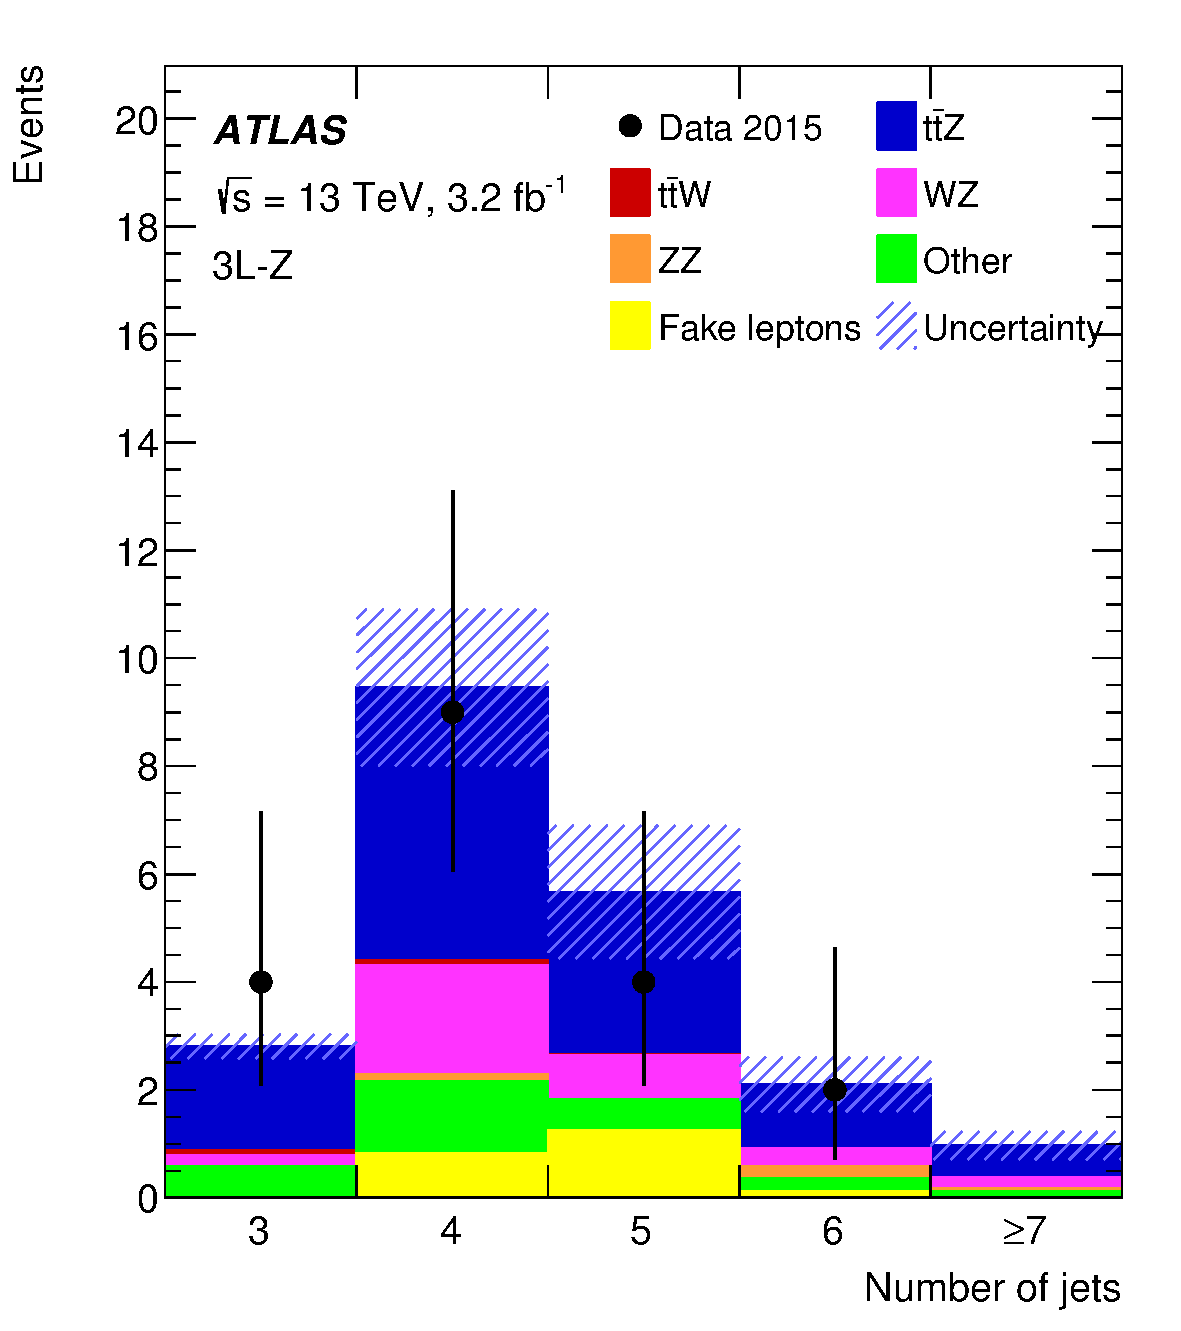
\includegraphics[width=\twofigwidth]{SR3lZnJets}
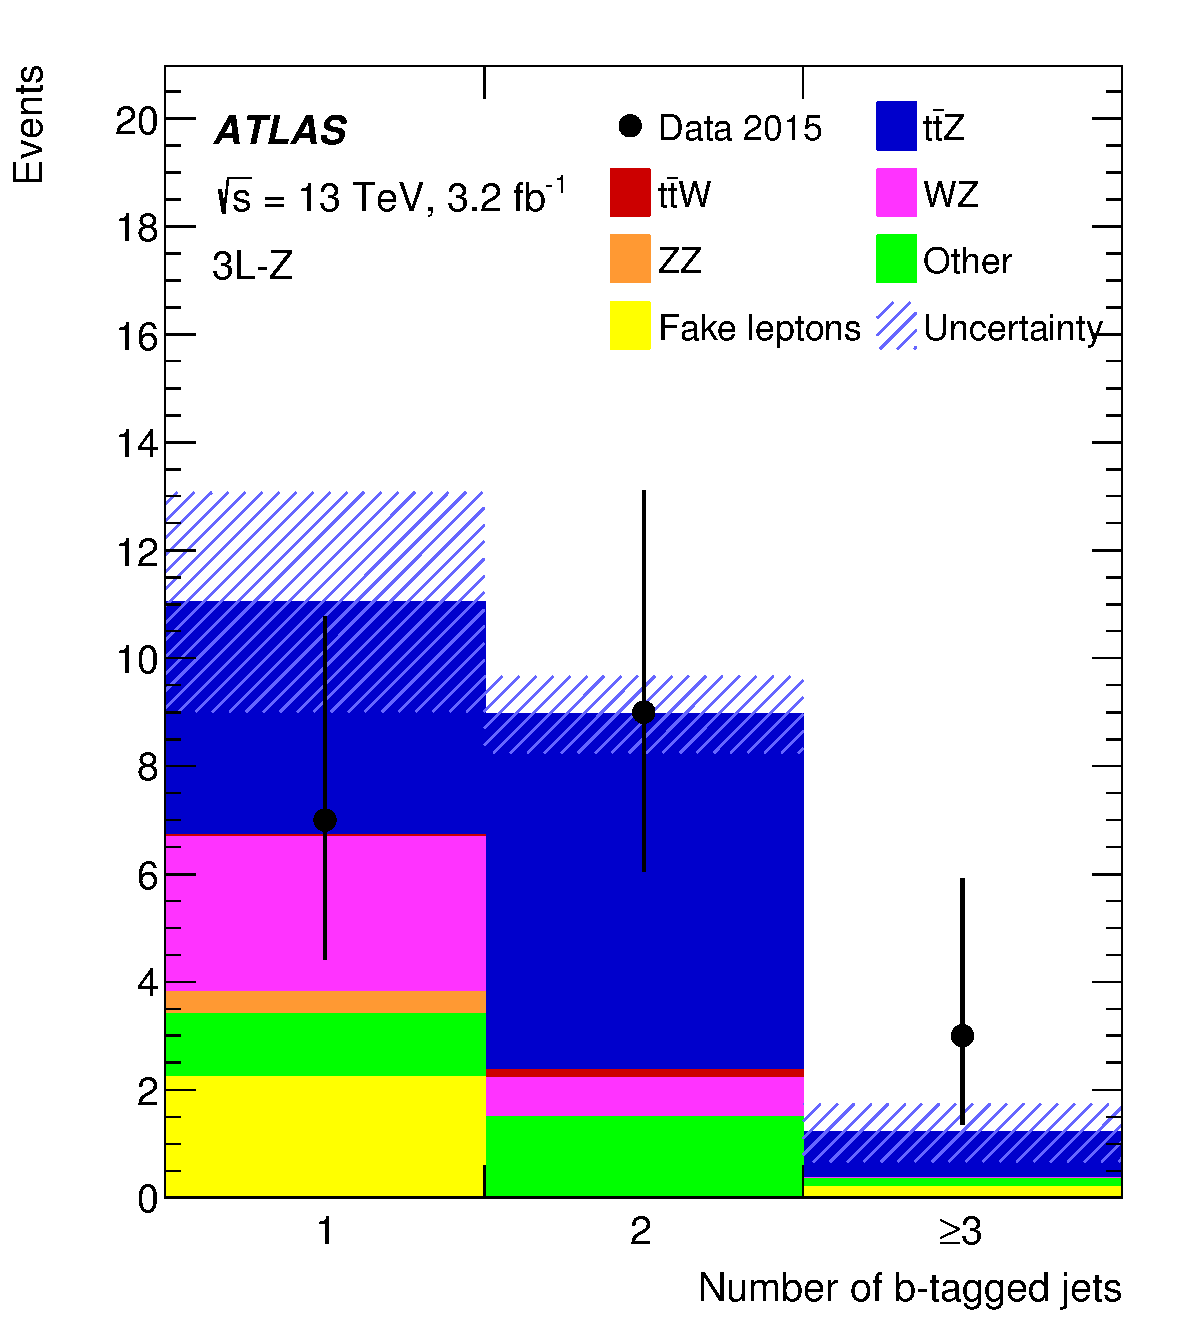
\includegraphics[width=\twofigwidth]{SR3lZnBJets}
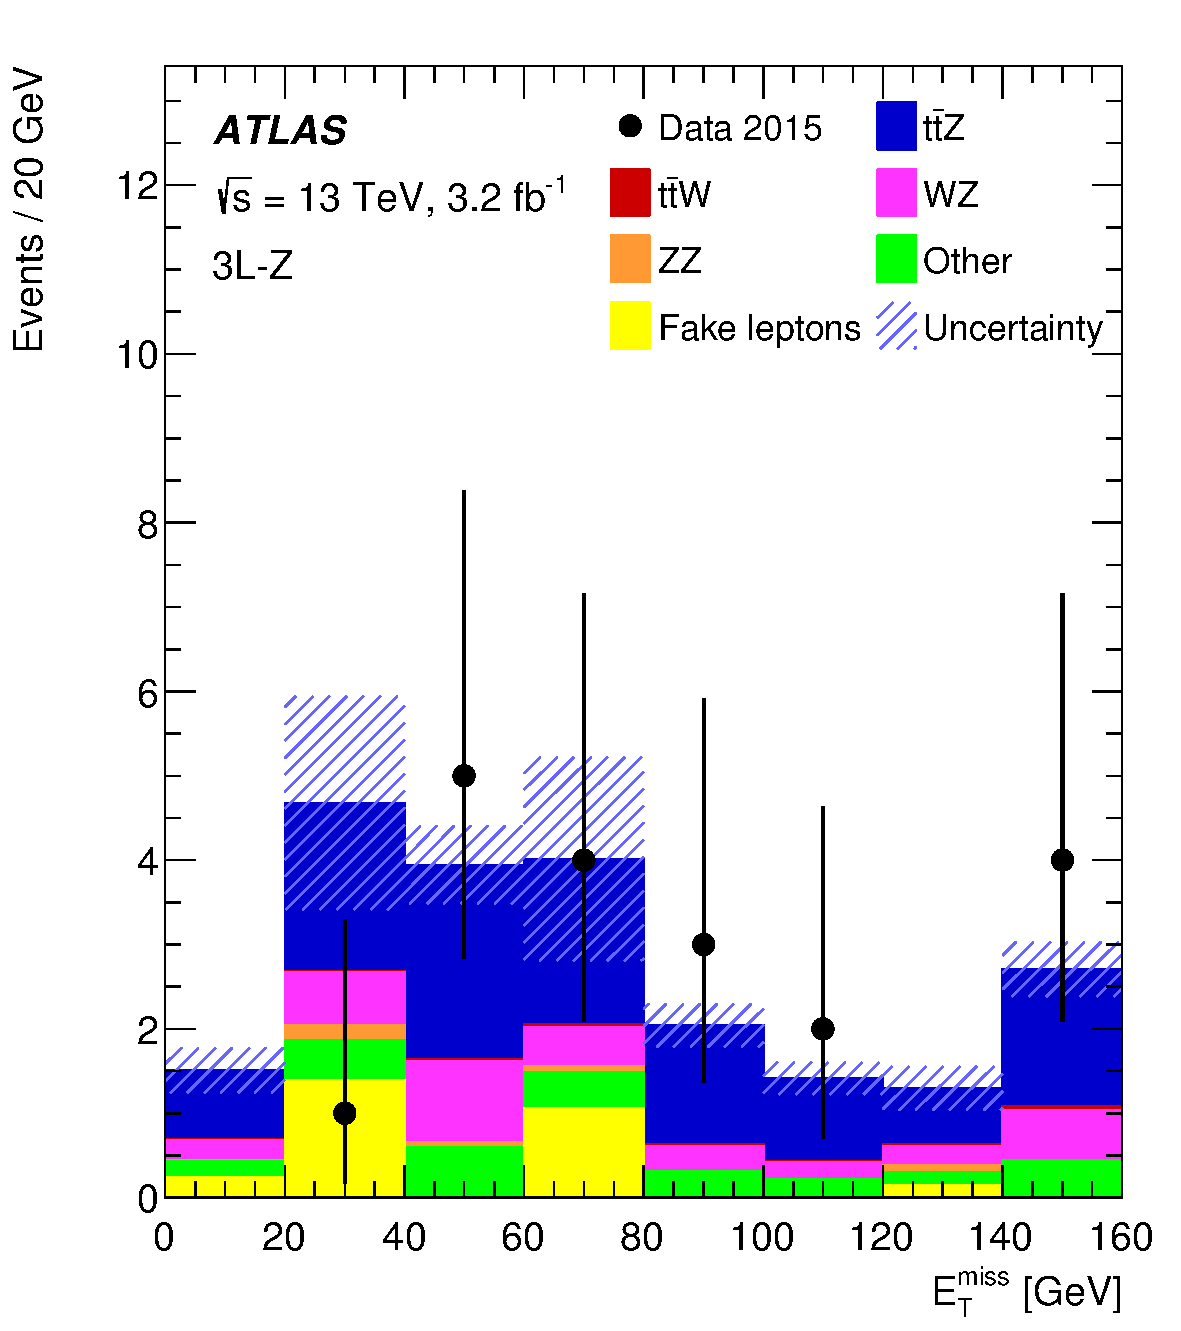
\includegraphics[width=\twofigwidth]{SR3lZMET}
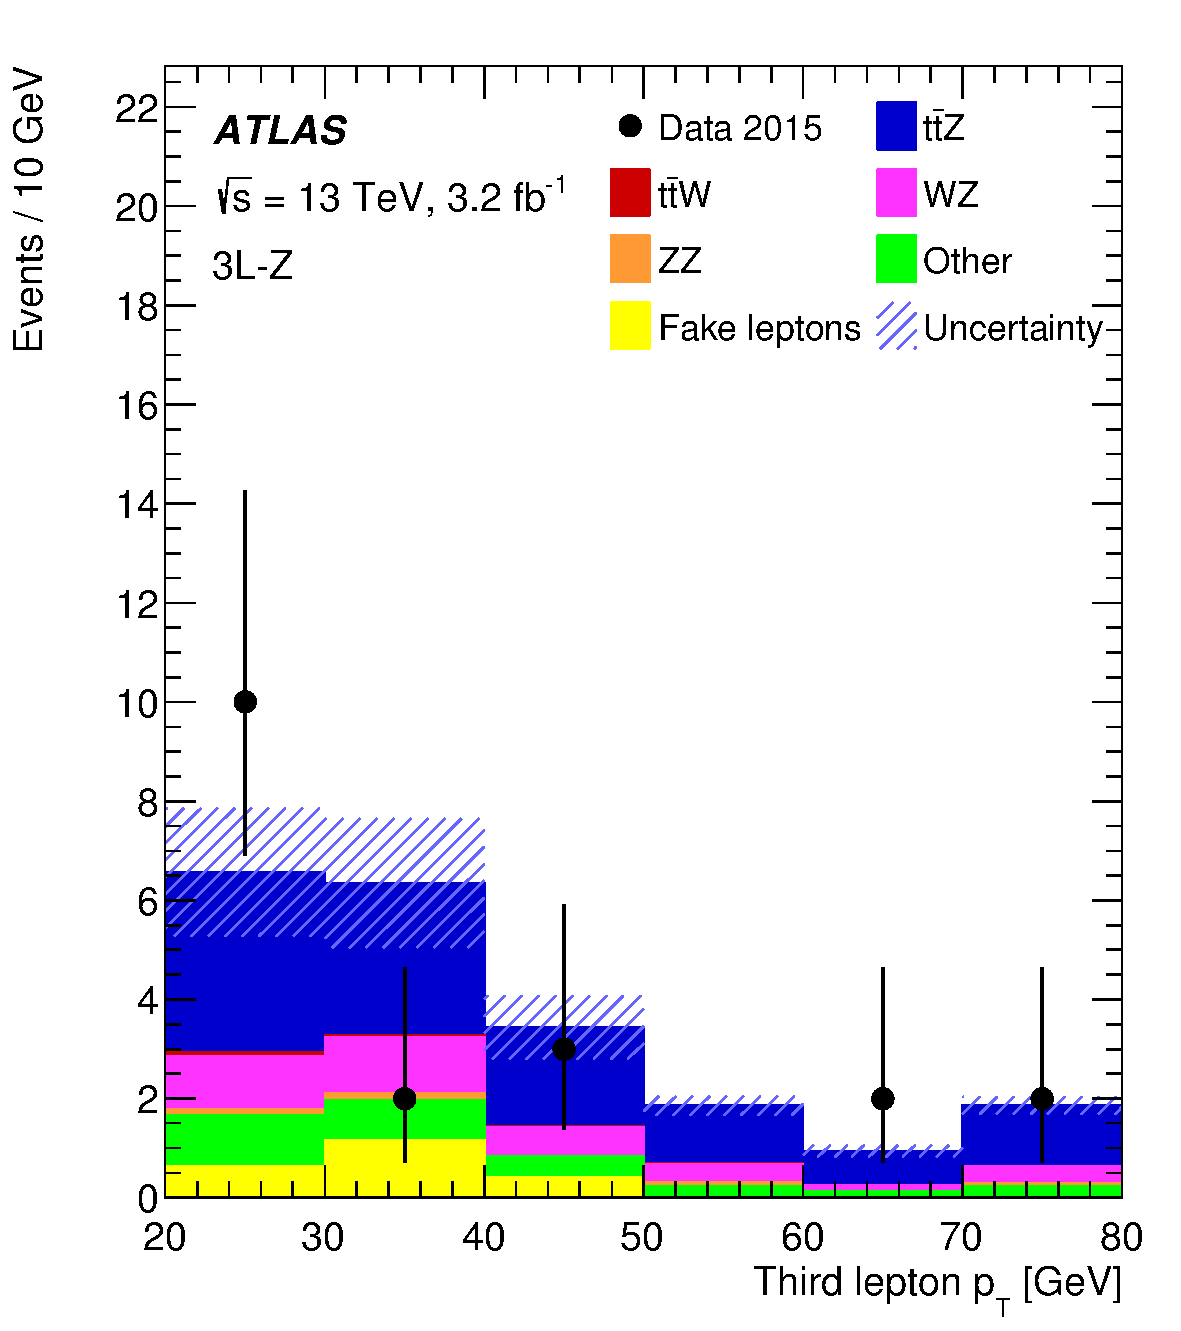
\includegraphics[width=\twofigwidth]{SR3lZpT3lep}
\caption{\label{fig:3l_sr} Distributions of (top left) the number of jets, (top
right) the number of $b$-tagged jets, (bottom left) the missing transverse
momentum and (bottom right) the third-lepton \pt, for events contained in any
of the three signal regions \TLSRA, \TLSRB\ or \TLSRC. The distributions are
shown before the fit.  The background denoted `Other' contains other SM
processes producing three prompt leptons.  \hatch. The last bin in each of the
distributions shown in the bottom panels includes the overflow.}
\end{figure}

\subsection{Tetralepton analysis}
\label{s:4L}

The \FLC\ targets the \ttZ process for the case where both $W$ bosons resulting
from top-quark decays and the $Z$ boson decay leptonically.  Events with two
pairs of opposite-sign leptons are selected, and at least one pair must be
of same flavour. The OSSF lepton pair with reconstructed invariant mass closest to
$m_Z$ is attributed to the \Zboson boson decay and denoted in the following by
$Z_1$.  The two remaining leptons are used to define $Z_2$.  Four signal
regions are defined according to the relative flavour of the two $Z_2$ leptons,
different flavour (DF) or same flavour (SF), and the number of $b$-tagged jets:
one, or at least two ($1b$, $2b$).  The signal regions are thus \FLSRB, \FLSRC,
\FLSRD\ and \FLSRE.

To suppress events with fake leptons in the 1-$b$-tag multiplicity regions, additional requirements on the scalar sum of the transverse momenta of the
third and fourth leptons ($\pttf$) are imposed.  In the \FLSRD\ and \FLSRB\
regions, events are required to satisfy $\pttf > \SI{25}{\gev}$ and $\pttf >
\SI{35}{\gev}$, respectively.  In all regions, the invariant mass of any two
reconstructed OS leptons is required to be larger than \SI{10}{\gev}. The signal region definitions for the \FLC\ are summarised in Table~\ref{tab:SRs4l}.

\begin{table}[htbp]
\centering \renewcommand{\arraystretch}{1.2}
\caption{\label{tab:SRs4l} Definitions of the four signal regions in the \FLC.
All leptons are required to satisfy \mbox{$\pT > 7\,\GeV$} and at least one lepton with
$\pt > 25\,\GeV$ is required to be trigger matched. The invariant mass of any two
reconstructed OS leptons is required to be larger than \SI{10}{\gev}.\vspace{1ex}}
\begin{tabular}{lccr@{}cc@{}lc}
\toprule  
Region & $Z_2$ leptons &  \pttf && $|m_{Z_{2}} - m_Z| $ & \met && $n_{b{\text{-tags}}}$\\
\midrule
\FLSRB & $e^{\pm}\mu^{\mp}$ & $>\SI{35}{\gev}$ &&-&-&& 1\\
\FLSRC & $e^{\pm}\mu^{\mp}$ & -&&-&-&& $\ge2$\\
\FLSRD & $e^{\pm}e^{\mp},\mu^{\pm}\mu^{\mp}$ & $>\SI{25}{\gev}$ & \begin{tabular}{@{}r@{}} \ldelim\{{2}{2ex} \\ \\ \end{tabular} &
\begin{tabular}{c}$>\SI{10}{\gev}$\\ $<\SI{10}{\gev}$\end{tabular} & \begin{tabular}{c}$>\SI{40}{\gev}$\\ $>\SI{80}{\gev}$\end{tabular} &\begin{tabular}{@{}l@{}} \rdelim\}{2}{2ex} \\ \\ \end{tabular} & 1\\
\FLSRE & $e^{\pm}e^{\mp},\mu^{\pm}\mu^{\mp}$ &-&\begin{tabular}{@{}r@{}} \ldelim\{{2}{2ex} \\ \\ \end{tabular} &
\begin{tabular}{c}$>\SI{10}{\gev}$\\ $<\SI{10}{\gev}$\end{tabular} & \begin{tabular}{c}-\\ $>\SI{40}{\gev}$\end{tabular} &\begin{tabular}{@{}l@{}} \rdelim\}{2}{2ex} \\ \\ \end{tabular} & $\ge2$ \\
\bottomrule 
\end{tabular}
\end{table}

A control region used to constrain the $ZZ$ normalisation, referred to as \FLCR, 
is included in the fit and
is defined to have exactly four reconstructed leptons, a \SecondZ\ pair with
OSSF leptons, the value of both \FirstZM\ and \SecondZM\ within $10\,\GeV$ of the
mass of the $Z$ boson, and $\met <40\,\GeV$. The leading lepton \pT, the 
invariant mass of the $Z_2$ lepton pair, the missing transverse momentum and the 
jet multiplicity in this control region are shown in Figure~\ref{fig:zz_val},
and good agreement is seen between data and prediction.

\begin{figure}[htbp]
\centering
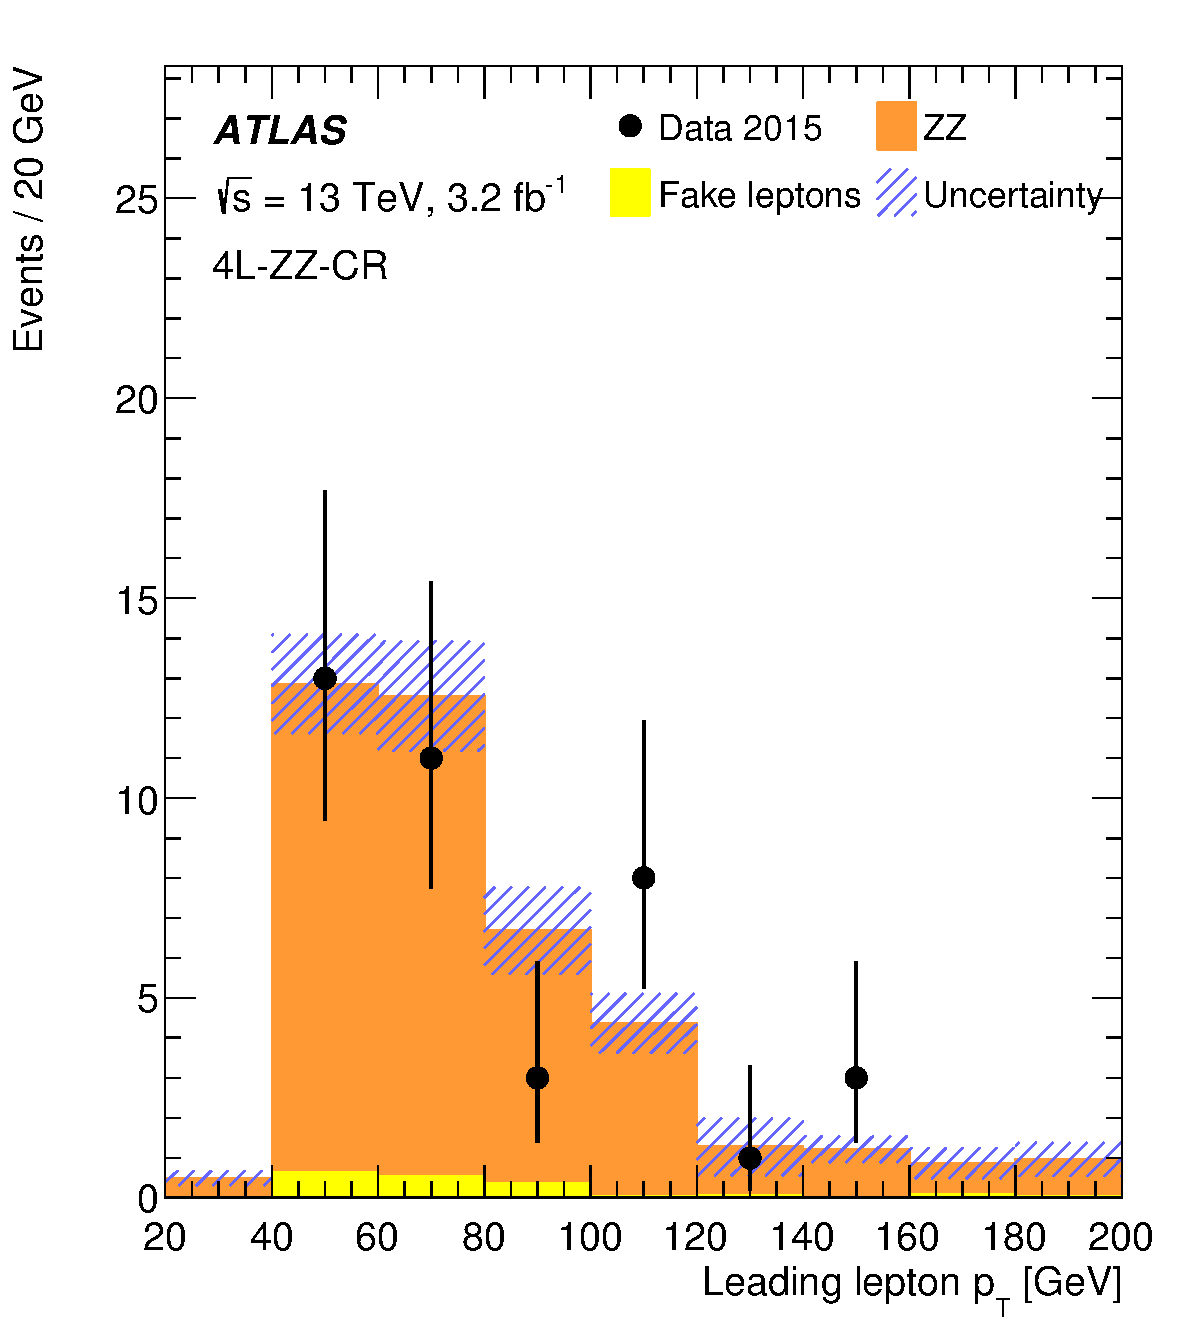
\includegraphics[width=\twofigwidth]{CRZZpT1lep}
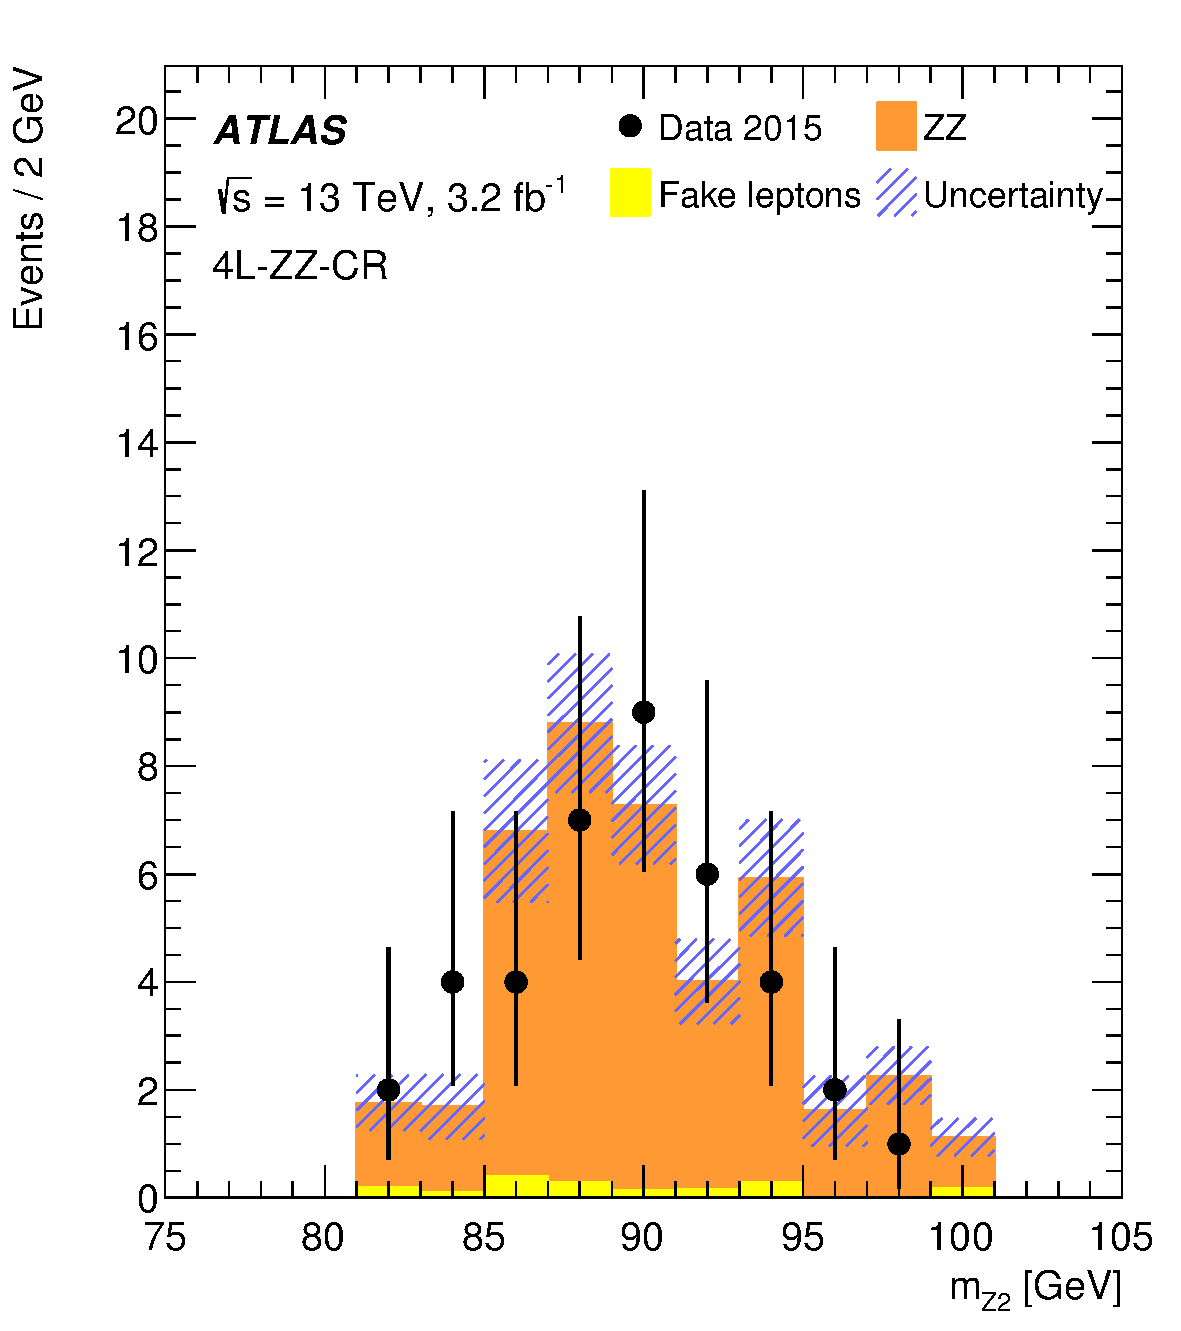
\includegraphics[width=\twofigwidth]{CRZZMZ2}
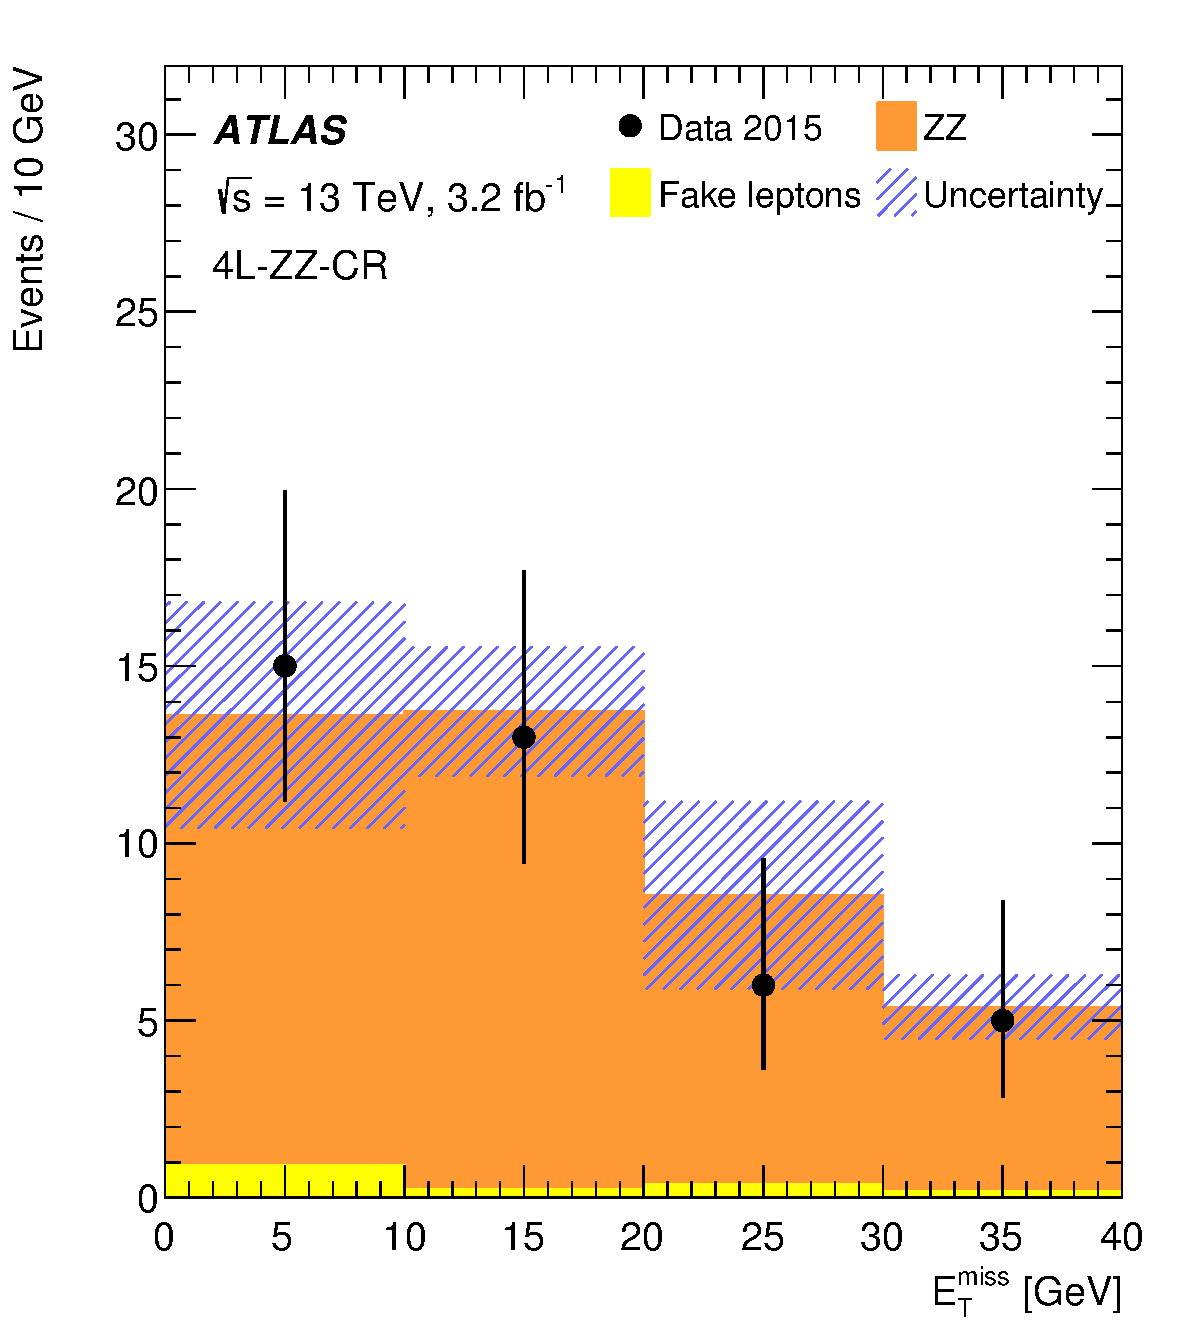
\includegraphics[width=\twofigwidth]{CRZZMET}
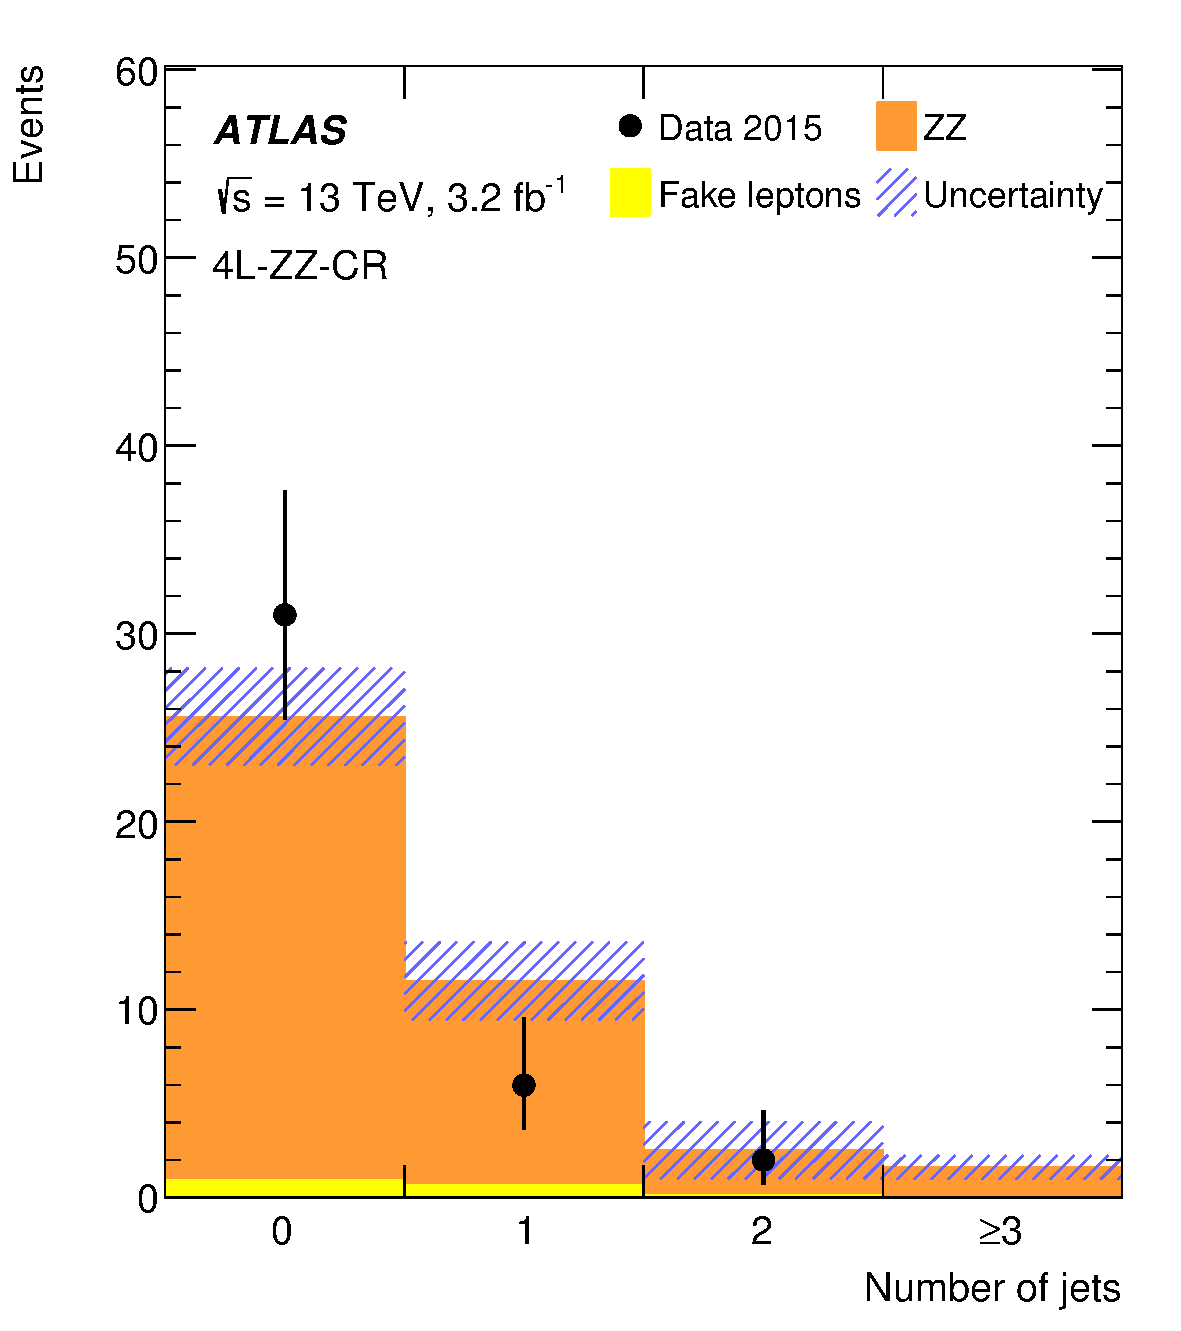
\includegraphics[width=\twofigwidth]{CRZZnJets}
\caption{\label{fig:zz_val} (Top left) Leading lepton \pt, (top right)
$m_{Z_2}$, (bottom left) missing transverse momentum and (bottom right) jet
multiplicity distributions in the \FLCR\ control region. The distributions are shown
before the fit. \hatch. The last bin of the distribution shown in the top left
panel includes the overflow.} 
\end{figure}

The contribution from backgrounds containing fake leptons is estimated from
simulation and corrected with scale factors determined in two control regions:
one region enriched in \ttbar events and thus in heavy-flavour jets, and one
region enriched in $Z$+jets events, and thus in light-flavour jets.  The scale factors
are calibrated separately for electron and muon fake-lepton candidates.  The
scale factors are applied to all MC simulation events with fewer than four
prompt leptons according to the number and the flavour of the fake leptons.
The \ttbar scale factors are applied to MC processes with real top quarks,
while for all other processes the $Z$+jets scale factors are applied. Different
generators are used when determining the scale factors and when applying them.
It is verified that the uncertainties in the scale factors include the differences between these generators.

The expected yields in the signal and control regions in the \FLC\ are shown
in Table~\ref{tab:yields}.  Five events are observed in the four signal
regions. Figure~\ref{fig:SR4l} shows the data superimposed to the expected
distributions for all four signal regions combined.
Overall the acceptance times efficiency for the \ttZ and \ttW
processes is 6\textperthousand\ and 2\textperthousand, respectively.  

\begin{figure}[htbp]
\centering
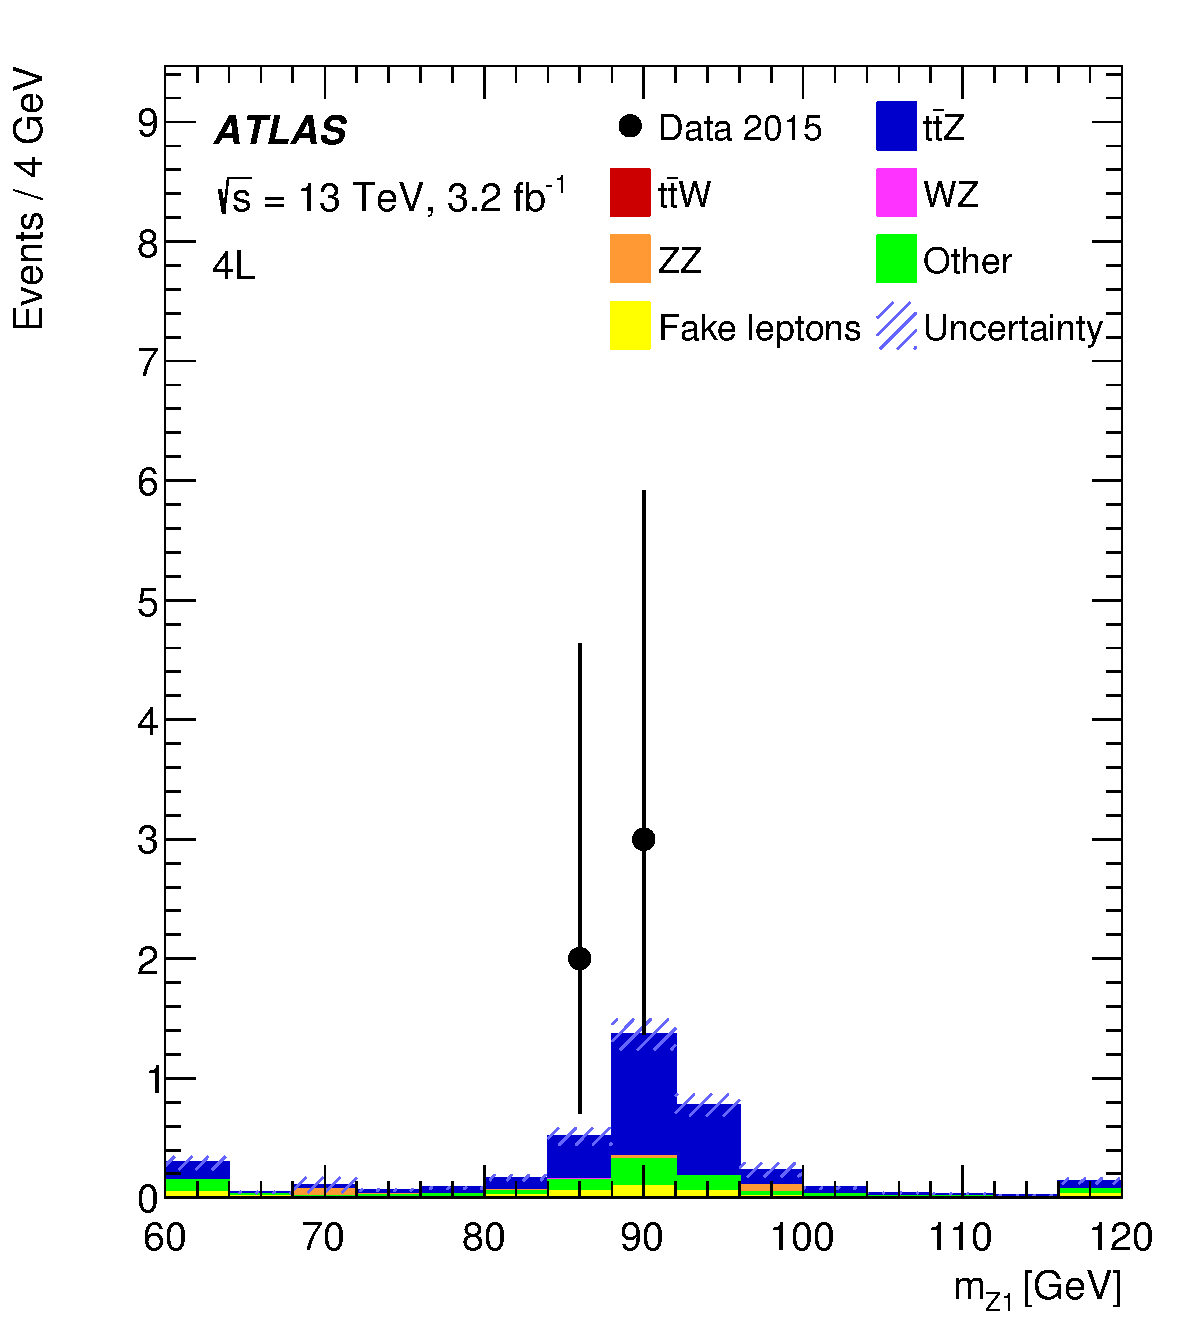
\includegraphics[width=\twofigwidth]{SR4lmll}
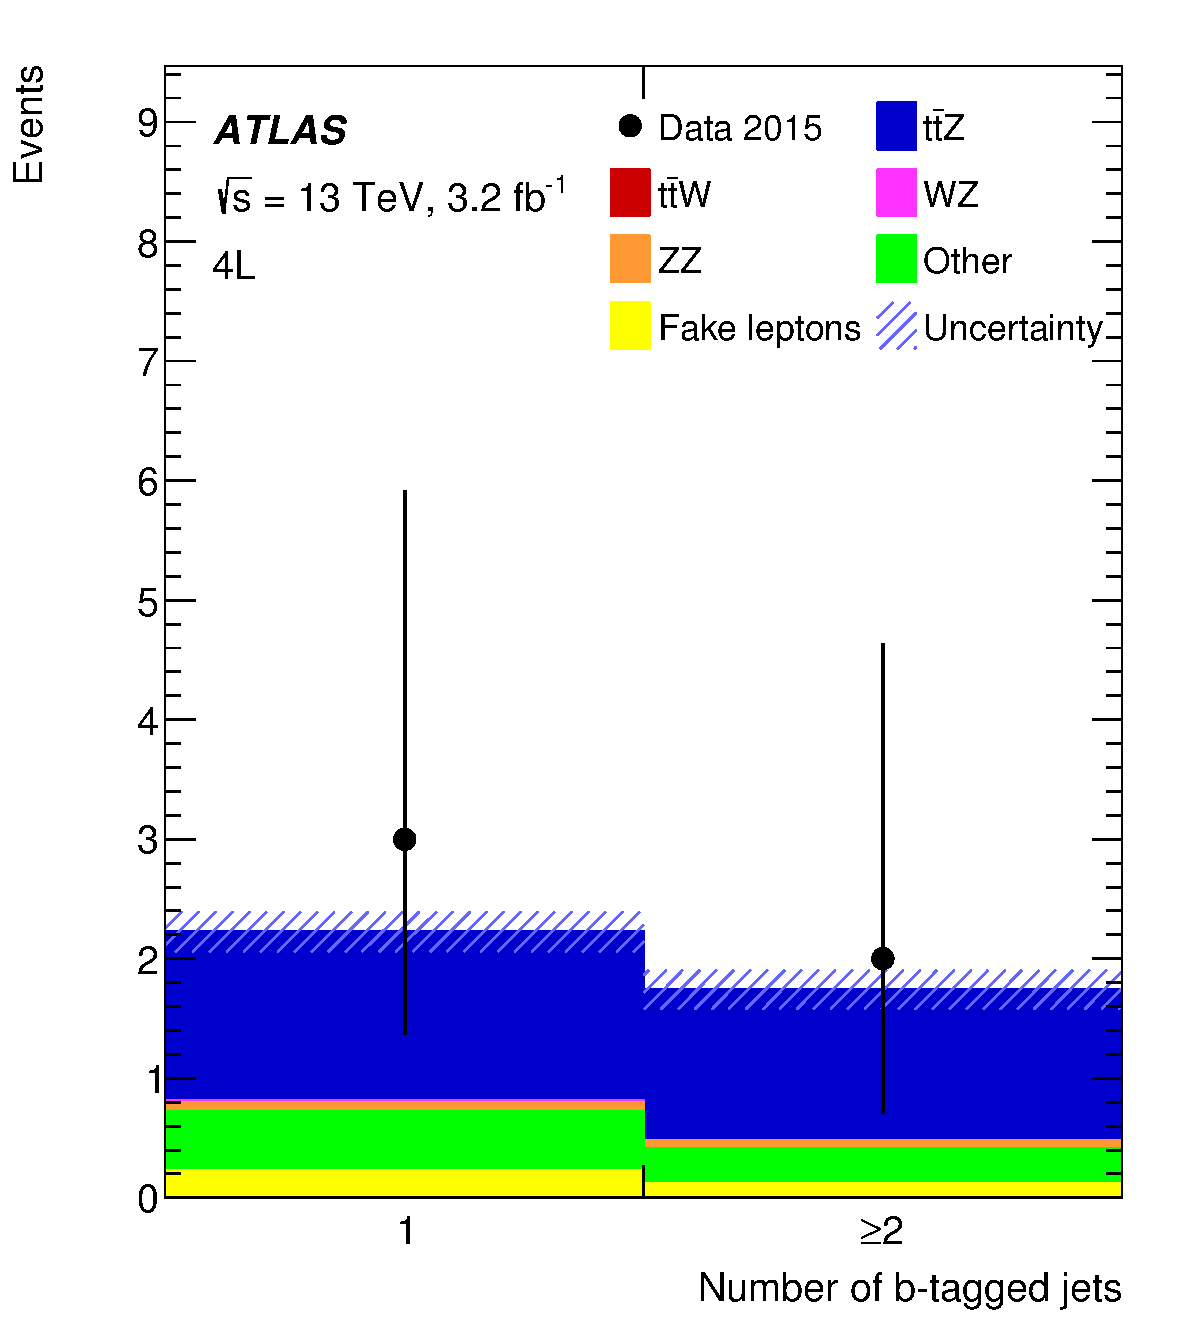
\includegraphics[width=\twofigwidth]{SR4lnBJets}
\caption{\label{fig:SR4l} Distributions (left) of the invariant mass of the
OSSF lepton pair closest to the $Z$ boson mass, $m_{Z_1}$, and (right) of the
number of $b$-tagged jets, for events in the tetralepton signal regions.  The
distributions are shown before the fit.  The background denoted `Other'
contains other SM processes producing four prompt leptons.  \hatch.  The first
and last bin of the distribution shown in the left panel include the underflow
and overflow, respectively.} 
\end{figure}

\begin{table}[htbp]
\centering \renewcommand{\arraystretch}{1.2}
\caption{\label{tab:yields} Expected event yields for signal and backgrounds,
and the observed data in all control and signal regions used in the fit to
extract the \ttZ and \ttW cross sections.  The quoted uncertainties in the expected
event yields represent systematic uncertainties including MC statistical
uncertainties.  The \tZ, \WtZ, \ttH, three- and four-top-quark processes are
denoted $t+X$. The $WZ$, $ZZ$, $H \to ZZ$ (ggF and VBF), $HW$ and $HZ$ and VBS
processes are denoted `Bosons'.
\vspace{1ex}}

\resizebox{\columnwidth}{!}{
\begin{tabular}{%
c|
r@{\,}@{$\pm$}@{\,}l
r@{\,}@{$\pm$}@{\,}l
r@{\,}@{$\pm$}@{\,}l
r@{\,}@{$\pm$}@{\,}l
|r@{\,}@{$\pm$}@{\,}l
r@{\,}@{$\pm$}@{\,}l
|r
}
\toprule
Region &
\multicolumn{2}{c}{$t+X$} &
\multicolumn{2}{c}{Bosons} &
\multicolumn{2}{c}{Fake leptons} &
\multicolumn{2}{c|}{Total bkg.} &
\multicolumn{2}{c}{\ttW} &
\multicolumn{2}{c|}{\ttZ} &
Data \\
\midrule
\TLCR&   $0.52$ & $0.13$&    $26.9$ & $2.2$&   $2.2$ & $1.8$&    $29.5$ & $2.8$& $0.015$ & $0.004$&   $0.80$ & $0.13$&    33\\
\FLCR&   \multicolumn{2}{c}{$<0.001$} &    $39.5$ & $2.6$&   $1.8$ & $0.6$& $41.2$ & $2.7$&    \multicolumn{2}{c}{$<0.001$} &    $0.026$ & $0.007$&    39\\
\midrule
\SSLSR&    $0.94$ & $0.08$&    $0.12$ & $0.05$&    $1.5$ & $1.3$&    $2.5$ & $1.3$&   $2.32$ & $0.33$&    $0.70$ & $0.10$&    9\\
\TLSRC&    $1.08$ & $0.25$&    $0.5$ & $0.4$&    \multicolumn{2}{c}{$<0.001$} & $1.6$ & $0.5$&   $0.065$ & $0.013$&    $5.5$ & $0.7$&    8\\
\TLSRA&    $1.14$ & $0.24$&    $3.3$ & $2.2$&    $2.2$ & $1.7$&    $6.7$ & $2.8$&   $0.036$ & $0.011$&    $4.3$ & $0.6$&    7\\
\TLSRB&    $0.58$ & $0.19$&    $0.22$ & $0.18$&    \multicolumn{2}{c}{$<0.001$} &    $0.80$ & $0.26$&    $0.083$ & $0.014$&    $1.93$ & $0.28$&    4\\
\TLSRD&    $0.95$ & $0.11$&    $0.14$ & $0.12$&    $3.6$ & $2.2$&    $4.7$ & $2.2$&   $1.59$ & $0.28$&    $1.45$ & $0.20$&    10\\
\FLSRD&    $0.212$ & $0.032$&    $0.09$ & $0.07$&    $0.113$ & $0.022$& $0.42$ & $0.08$&   \multicolumn{2}{c}{$<0.001$} &    $0.66$ & $0.09$&    1\\
\FLSRE&    $0.121$ & $0.021$&    $0.07$ & $0.06$&    $0.062$ & $0.012$& $0.25$ & $0.07$&   \multicolumn{2}{c}{$<0.001$} &    $0.63$ & $0.09$&    1\\
\FLSRB&    $0.25$ & $0.04$&    $0.0131$ & $0.0032$&    $0.114$ & $0.019$& $0.37$ & $0.04$&   \multicolumn{2}{c}{$<0.001$} &    $0.75$ & $0.10$&    2\\
\FLSRC&    $0.16$ & $0.05$&    \multicolumn{2}{c}{$<0.001$} &    $0.063$ & $0.013$&   $0.23$ & $0.05$&    \multicolumn{2}{c}{$<0.001$} &    $0.64$ & $0.09$&    1\\
\bottomrule
\end{tabular}
}
\end{table}
